\section{System Analysis and Design}
\label{sec:design}

This section outlines the high-level design of the Electronic Library Management System, covering the functional requirements, the software architecture, and the static structure of the core classes.

\subsection{Functional Requirements}
The system is designed to fulfill a comprehensive set of functional requirements, enabling efficient management of library operations. The core functionalities are:

\begin{itemize}
    \item \textbf{User Authentication:} Provides secure registration and login mechanisms for both Members and Librarians.
    \item \textbf{Book Management:} Supports full CRUD (Create, Read, Update, Delete) operations for the library's book collection.
    \item \textbf{Search Functionality:} Allows users to search the book catalog by title, author, and category, facilitating easy resource discovery.
    \item \textbf{Loan Management:} Manages the entire lifecycle of a book loan, including borrowing, returning, tracking loan status (active, returned, overdue), and calculating fines for overdue items.
    \item \textbf{User Account Management:} Enables librarians to manage member accounts and allows members to view their profiles and loan history.
    \item \textbf{Data Integrity:} Implements a CSV file hashing and verification mechanism to protect against unauthorized data tampering.
    \item \textbf{Notification System:} Capable of notifying users about important events, such as impending loan due dates.
\end{itemize}

\subsection{System Architecture}
The application employs a modular architecture to separate concerns and enhance maintainability\cite{Martin2017}. The codebase is organized into logical components, each with a distinct responsibility:

\begin{description}
    \item[\texttt{core/}] This directory contains the domain models, which represent the fundamental entities of the system. Key classes include \texttt{Book}, \texttt{User}, \texttt{Member}, \texttt{Librarian}, and \texttt{Loan}.
    \item[\texttt{services/}] This component encapsulates the primary business logic. It includes service classes like \texttt{LibraryManager} (which acts as a central facade for library operations), \texttt{AuthManager} for handling authentication, and \texttt{NotificationService}.
    \item[\texttt{patterns/}] Contains the implementations of the software design patterns used throughout the project, such as \texttt{Observer}, \texttt{Strategy}, and \texttt{Decorator}. This isolates pattern-specific code.
    \item[\texttt{utils/}] Provides various utility classes that support the core application logic. This includes the \texttt{CSVHandler} for data persistence, date utilities, and input validators.
    \item[\texttt{data/}] This directory serves as the data storage layer, containing the CSV files (\texttt{books.csv}, \texttt{members.csv}, etc.) that the application uses for data persistence.
\end{description}

\subsection{UML Core Class Diagram}
The static structure of the system is visualized in the UML Core Class Diagram below \cite{Booch2007} (Figure \ref{fig:class_diagram}). It illustrates the key classes, their attributes, methods, and the relationships between them, such as inheritance and association.

\begin{figure}[H]
    \centering
    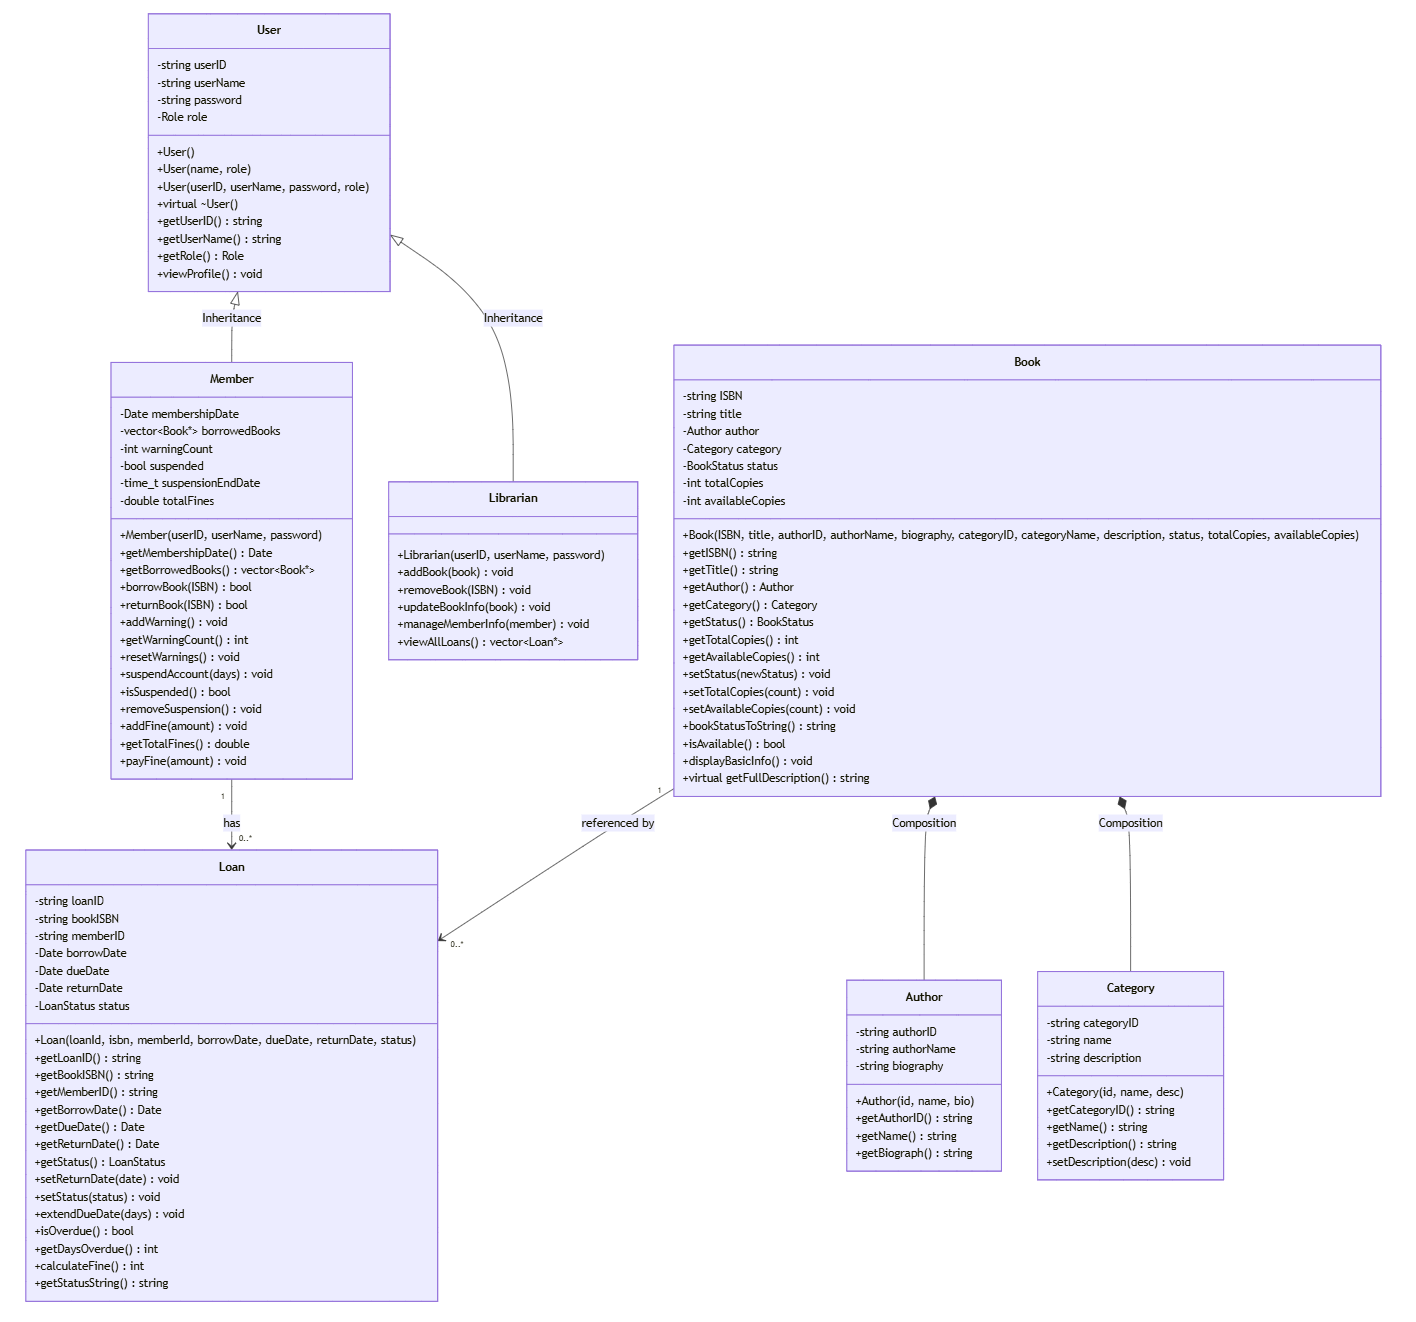
\includegraphics[width=\textwidth]{figures/class_diagram.png}
    \caption{UML Core Class Diagram of the Library Management System.}
    \label{fig:class_diagram}
\end{figure}